\documentclass[10pt,a4paper]{article}

\usepackage{graphicx}
\usepackage[utf8]{inputenc}
\usepackage[T1]{fontenc}  
\usepackage[english]{babel}
\usepackage{verbatim}
\usepackage{amsmath}
\usepackage{enumerate}
\usepackage{latexsym}
\usepackage{pdfpages}
\usepackage{ifthen}
\newboolean{paper}
\setboolean{paper}{false}

\begin{document}

\title{Team Report : ECMM409 - CA3}
\author {Deep Blue}
\date{\today}

\maketitle

\tableofcontents
\newpage

\section*{Introduction}
\addcontentsline{toc}{section}{Introduction}

As part of the ECMM409 team project, we decided to work on one of the
GECCO 2007 competition problems : Ant Wars.\\

This game, involving two opponent ants, takes place on a square
toroidal grid of dimension 11x11. Initially, 15 pieces of food are
randomly generated and placed on the game board. The respective
initial coordinates of the ants are (5, 2) and (5, 8). Playing
successively, the ants are allowed to move one step in every direction
including diagonal movements : (NW, N, NE, E, SE, S, SW, W). If an ant
enters a cell containing a piece of food, a point is added to its
score, however if ant enters the adverse cell, the opponent is killed
and cannot play anymore. The game lasts at most 35 moves per
player. The score being only based on the number of pieces of food
eaten, the ants have to collect as much food as possible from their
environment.\\

The aim of this project was to find the best ant algorithm we could,
using a nature inspired approach. We decided to use a strongly-typed
genetic programming algorithm to design our ant.\\

First, this short report will analyse and explain the choice of
genetic programming amongst the numerous nature inspired algorithms to
design our artificial ant. Then, the details of the algorithm will be
presented, followed by an explanation on the framework's
characteristics, implemented using Haskell. Finally, the results of
our computations will be presented.

\section{Road Map}

From the onset of the project, a road map was defined, clearly
identifying the important steps that would have to be completed. Of
course, this list of tasks was slightly updated throughout the
project, to take into account some difficulties related to the
implementation or to the unexpected results of some experiments.

\begin{itemize}
\item implement the framework
\item find and implement rule-based ants
\item run experiments on the ants, evaluate the performances with a tournament
\item implement a memory module to the ants and test its influence on the performances
\item design and implement a genetic programming algorithm
\item conduct experiments on the algorithm parameters
\item graphs on the evolution of the best genetic ant, generation after generation
\item evaluate the competitiveness of our best solution against
  rule-based ants and human players.
\end{itemize}

\section{Choice of nature inspired algorithm}

The GECCO web-page stipulates that the solution had to be evolved,
implying that genetic programming had to be used. However, in the
context of this project we had to consider every nature inspired
technique. The next paragraph lists the different nature inspired
techniques we were told and studied this term and why we think that
they were not appropriate to solve this problem :

\begin{itemize}
\item Cellular automaton : used to model phenomena
\item Neural network : input : grid - output : go forward or not |
  problem : huge set of training data needed
\item Genetic \amp PSO algorithm : for optimisation problems, exploring solution space
\end{itemize}

Only two approaches seemed to be possible. We could have evolved a
population of neural networks represented by a list of coefficients
using a genetic algorithm, each neural network representing an ant
taking a grid as input and calculating whether or not the ant should
go forward. But a genetic programming algorithm appeared to be more
natural approach to solve the ant wars problem.

\section{Genetic programming algorithm details}

Genetic programming is merely a genetic algorithm with programs
usually represented in the infix form using a tree structure.\\

We a used strongly-typed approach for our algorithm. In effect, the
trees were generated according to a predefined grammar and contained
two types of data : Boolean and integer values. The operators used
were functions manipulating these two types and were inspired by some
rule-based ant algorithm we had previously designed.\\

The grammar was defined by :
\begin{itemize}
\item B expression
  \begin{itemize}
    \item T : represent true value 
    \item F : represent false value
    \item IsFood Rect : is there food in the specified rectangular area?
    \item IsEmemy Rect : is there an enemy?
    \item And B B
    \item Or B B
    \item Not B
    \item IsSmaller I I
    \item IsEqual I I
  \end{itemize}
\item I expression
  \begin{itemize}
  \item Const Int : represent an integer value
  \item If B I I
  \item Add I I
  \item Sub I I
  \item Mul I I
  \item NbFood Rect : number of pieces of food within the area specified
  \item NbEmpty Rect : number of empty cells
  \item NbVisived Rect : number of cells already visited
  \item Point : pieces of food eaten so far
  \item PointLeft : potential number of food left on the grid
  \item TimeLeft : number of turn before the game ends
  \item FoodHope Rect : number of pieces of food accessible within two moves
  \end{itemize}
\end{itemize}

An ant was represented by two I expressions. Indeed, to exploit the
symmetry of the game, the first tree was evaluated to generate an
integer which represented the likeliness to go North, then the grid was
rotated and presented again to the tree to be evaluated. The second
tree represented a diagonal movement on the grid. After evaluating the
height possibilities, the ant selects the direction associated with
the higher number computed.\\

What differs from usual genetic algorithm is that we are not using any
explicit fitness function to evaluate the population of ants. Indeed,
a fitness function associates a number characterising the performances
of a particular individual, in our case one cannot assess the
performance of a given ant without playing games against other
ants. This was quite problematic, so we decided to combine the
selection and evaluation step in one phase to avoid the problem of
finding a fitness function.\\

To generate a new individual given a population, we randomly select a
certain number of ants according to a pressure parameter without
removing them from the population, then these ants are playing a match
against each other in a simple tournament in order to find the best
ant of the selected group. The process is repeated to find a second
ant. Given these two ants, the traditional crossing-over and mutation
operators are applied to give two evolved ants. Finally, we repeat
the precedent step a sufficient number of time until the size of the
population is reached.\\

The key differences are that there is no fitness function, the
selection and evaluation steps are combined, a whole new population is
created at each step of the algorithm.\\

Last, when the termination criteria is met, a round-robin tournament
is played to determine the best ant of lastly evolved population. This
particular ant is then declared to be the result of our algorithm.

\section{Framework and algorithm implementation}

We used Haskell, a functional programming language, to implement the
game framework as well as the genetic algorithm.\\

Two of most important features characterising Haskell are its laziness
and strongly typed system. The former was extremely useful and justify
the use of Haskell for the implementation : the grammar we defined was
explicitly recursive, and thus Haskell's laziness allowed us to
defined mutually recursive data structure to represent the grammar. On
the other side, the strong type system happened to be extremely useful
to define functions manipulating the tree expressions such as the
mutation operators.

\section{Results}

The best evolve ant can be found in the experiment directory
(experiment \slash standard\_island4\_37.ant)\\

As Figure \ref{food} suggests, generation after generation the average
level of the population increase, and by the end of the algorithm, 13
out 15 pieces of food were find by the competing ants.\\

\begin{figure}
\begin{center}
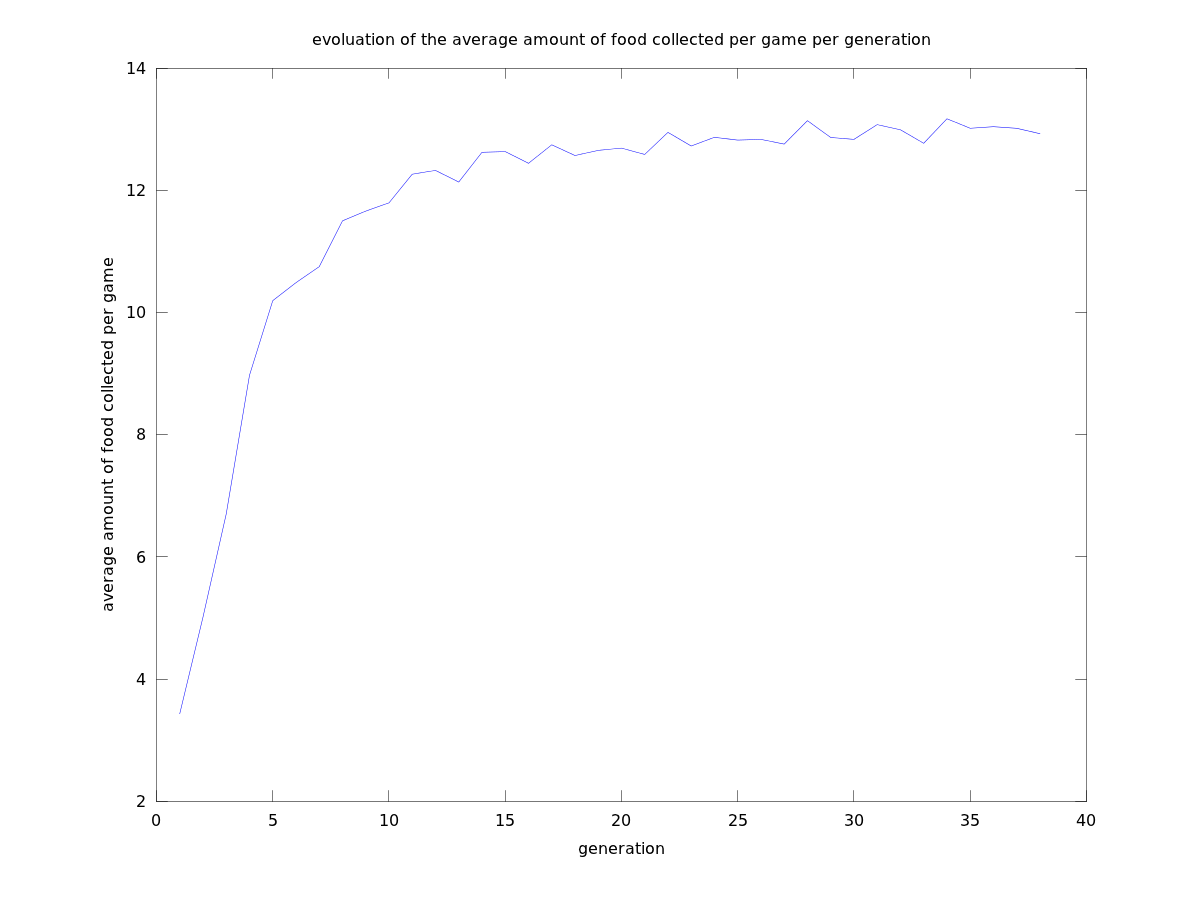
\includegraphics[scale=0.3]{../experiment/standard_island4_food_stat.png}
\end{center}
\label{food}
\end{figure}

However, the best ant we could evolved was less victorious than most
of rule-based ants we designed. This is showed by Figure \ref{rules}

\begin{figure}
\begin{center}
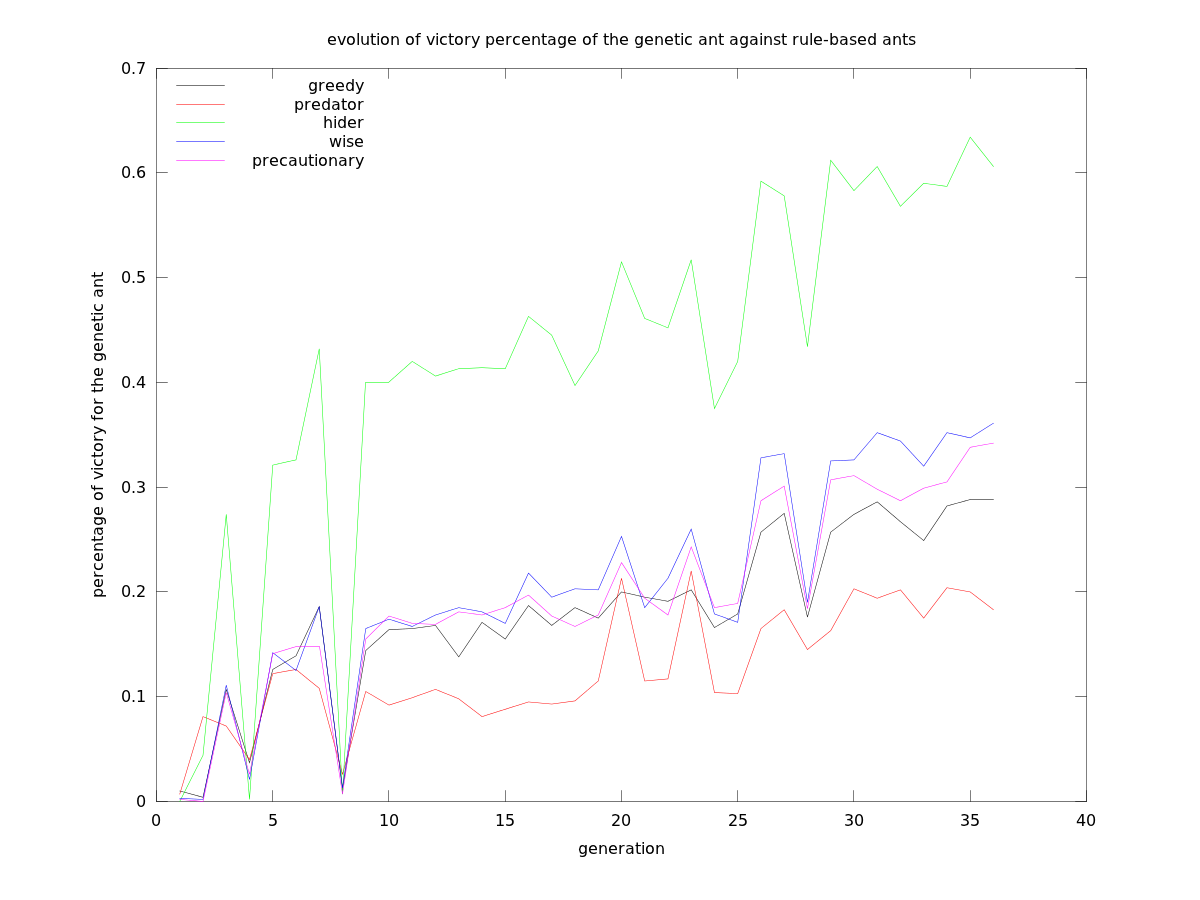
\includegraphics[scale=0.3]{../experiment/standardBestAnt.png}
\end{center}
\label{rules}
\end{figure}

\section*{Conclusion}
\addcontentsline{toc}{section}{Conclusion}

So far, we did not manage to evolve ants more efficient than
manually-designed rule-based ants. However it can be easily seen that
our genetic algorithm tend to produce better ants generation after
generation

\end{document}
